\begin{figure}[t]
\begin{center}
\begin{small}
\begin{sc}
\begin{tabular}{c@{\hskip2pt}c@{\hskip2pt}c@{\hskip2pt}c}
Image&Target&Ours&GlAtEx\\
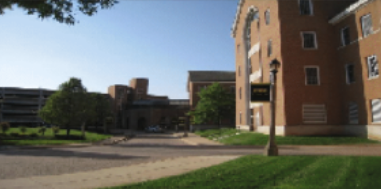
\includegraphics[width=\smallimg]{fig/seg/1/img.png}&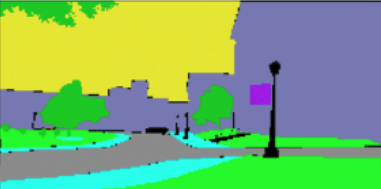
\includegraphics[width=\smallimg]{fig/seg/1/gt.png}&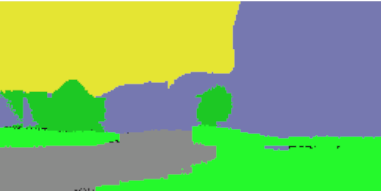
\includegraphics[width=\smallimg]{fig/seg/1/ours.png}&
\includegraphics[width=\smallimg]{fig/seg/1/glatex.png}\\

\includegraphics[width=\smallimg]{fig/seg/2/img.png}&
\includegraphics[width=\smallimg]{fig/seg/2/gt.png}&
\includegraphics[width=\smallimg]{fig/seg/2/ours.png}&
\includegraphics[width=\smallimg]{fig/seg/2/glatex.png}\\

\includegraphics[width=\smallimg]{fig/seg/3/img.png}&
\includegraphics[width=\smallimg]{fig/seg/3/gt.png}&
\includegraphics[width=\smallimg]{fig/seg/3/ours.png}&
\includegraphics[width=\smallimg]{fig/seg/3/glatex.png}\\

\includegraphics[width=\smallimg]{fig/seg/4/img.png}&
\includegraphics[width=\smallimg]{fig/seg/4/gt.png}&
\includegraphics[width=\smallimg]{fig/seg/4/ours.png}&
\includegraphics[width=\smallimg]{fig/seg/4/glatex.png}\\
\end{tabular}
\end{sc}
\end{small}
\end{center}
\vskip -0.1in
\caption{\textbf{Segmentation quality for ADE20K:} Semantic segmentation results of our method compared with GlAtEx~\protect\cite{seifi2021glimpse} on the ADE20k dataset. Qualitatively, segmentation maps produced by our method are at least as good as those of the competition.}
\label{fig:qualiative-seg}
\end{figure}